\documentclass{article}
\usepackage{graphicx} % Required for inserting images
\title{AMATYC J-4}
\author{Curtis Bradley}
\usepackage{graphicx}
\usepackage{titling}
\usepackage{amssymb}
\begin{document}
\setlength{\droptitle}{-4cm}
\maketitle

\section{Problem} Start with a regular hexagon of side 1 as level 1. At each level $n -1$, form the regular hexagon of level $n$ by joining consecutive midpoints of the one for level $n-1$. Find the lowest level at which the associated regular hexagon has a perimeter under 1.
\section{Solution}
Construct a regular hexagon with side length $S_k$, such that the perimeter $P_k = 6S_k$. 
Construct a second hexagon inscribed in the first with vertices intersecting the first's midpoints. 
Observe that six identical triangles are made between both hexagons with side lengths of the triangle of $\frac{S_k}{2}$ separated by an angle of $120^\circ$ (the interior angle of the hexagon). 
Using law of cosines, the side length of the inscribed hexagon can be found to be  $S_{k+1} = \frac{\sqrt{3}}{2}S_k$. 
We can construct an equation for $P_k$ as such:
\[P_k = 6 S_1 \cdot\left(\frac{\sqrt{3}}{2}\right)^{k-1}\]
Setting $P_k$ to 1 and $S_1$ to 1, it can be found $k=1 + \frac{\ln{6}}{\ln{\frac{2\sqrt{3}}{3}}} \approx 13.45$. Therefore the smallest integer level $n$ where $P_n \leq 1$ is $n = \lceil{k}\rceil = 14$ where $P_{14}\approx0.92$.$\square$


\begin{center}
    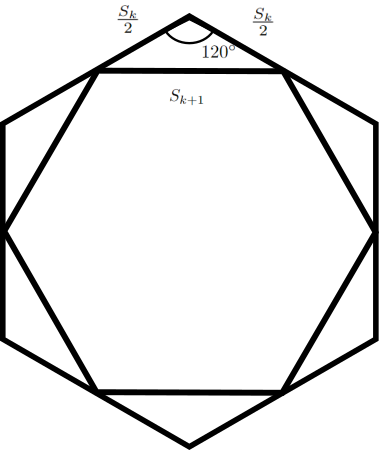
\includegraphics[scale=0.5]{hexagon.png}

    Diagram of hexagon with side lengths $S_k$ with inscribed hexagon of side lengths $S_{k+1}$
\end{center}
\end{document}

